\chapter{Introdução} \label{chapter:introduction}
% O conceito de ensinar uma máquina, ou um conjunto delas, a realizar tarefas que requerem a capacidade do pensamento humano e raciocínio data da antiguidade. Na Ilíada de Homero \cite{homero2015}, o deus Hefesto, considerado deus da tecnologia, cria máquinas humanoides de bronze com o objetivo de auxiliá-lo a se movimentar. Entretanto, a criação da inteligência artificial (IA) nos moldes atuais é atribuída a Alan Turing, quando o mesmo propôs o conhecido ``teste de Turing'' como uma medida da inteligência de máquina.

% A inteligência humana tem despertado curiosidade há mais de dois milênios.   O campo de inteligência artificial (IA) nasce a partir de uma combinação de diferentes ideias provenientes de trabalhos, em grande maioria, destas áreas. 
% O processo de aprendizagem humano é tão complexo que definir o termo aprendizagem torna-se difícil.
% Desde o surgimento dos computadores houveram especulações acerca da possibilidade de ensiná-los a realizar tarefas inteligentes.
% A inteligência é um termo complexo e definí-lo precisamente mostra-se um trabalho árduo. Mais especificamente,
% A competência que o ser humano demonstra na realização de atividades como reconhecimento de objetos e comunicação via elaborados sistemas de linguagens sempre
% O estudo sobre aprendizagem e inteligência é uma das disciplinas mais antigas
% A competência que o ser humano apresenta na realização de atividades como reconhecimento de objetos e comunicação via elaborados sistemas de linguagens o difere dos demais seres vivos.
% O ser humano, graças à sua capacidade mental, possui habilidades únicas que o difere dos demais seres vivos.
% Reconhecimento visual de objetos, comunicação via elaborados sistemas de linguagens e extrema competência em disciplinas científicas são alguns exemplos que mostram o potencial de aprendizagem e evolução.
% A capacidade de aprender, em linhas gerais, é um objeto de
% A capacidade de aprender do ser humano é um objeto de estudo que desperta interesse e intriga pesquisadores de diversas áreas de pesquisa, como filosofia, psicologia, neurociência etc. Aprendizagem, assim como inteligência, abrange um vasto conjunto de processos interoperantes de uma maneira tão complexa que torna difícil de ser definida. Habilidades singulares, tais como reconhecimento visual de objetos, comunicação via elaborados sistemas de linguagens e a criação de complexos teoremas nas mais difíceis disciplinas, são apenas alguns exemplos que mostram como o constante processo de aprendizado torna nossa espécie tão única.
% Por centenas de anos, muito foi estudado acerca de como o processo de aprendizagem do cérebro humano funciona. Entretanto, a inteligência artificial (ou IA) busca não somente entender como funciona, mas também construir entidades que tenham habilidade de aprender \cite{Russell:2009:AIM:1671238}.

As capacidades cognitivas características do ser humano despertam interesse e curiosidade há séculos. O modo como percebemos, entendemos e manipulamos o mundo à nossa volta tem nos destacado dos demais seres vivos, de modo a nos classificar como seres racionais. A busca pelo conhecimento acerca de nossas tomadas de decisões (inteligentes) abrange áreas de estudo tais como filosofia, matemática, psicologia e fisiologia. De fato, uma mescla dessas áreas decorreu na criação do campo de Inteligência Artificial (IA). Entretanto, o objetivo da IA transcende aos de seus gestores pois esforça-se não somente em entender entidades inteligentes, como também construí-las \cite{russell2009}.

Apesar de não haver concordância sobre a definição universal do termo ``inteligência'', pode-se encontrar muitas similaridades entre as diversas existentes, tais como a recorrência dos termos conhecimento e aprendizado. Com o intuito de criar entidades inteligentes, muitos paradigmas de aprendizado foram propostos à medida que as pesquisas em IA foram amadurecendo. Um dos principais é o aprendizado indutivo, um processo de aquisição de conhecimento através da extração de inferências indutivas fornecidas por um professor/instrutor ou ambiente externo.

Ao aperfeiçoamento do desempenho de um agente inteligente na realização de uma determinada tarefa por meio da experiência é dado o nome de Aprendizado de Máquina (AM) \cite{mitchell1997}. Mais particularmente, o processo que induz um agente inteligente a aprender como realizar com êxito determinada tarefa se dá através da existência de exemplos na forma (\textit{entrada}, \textit{saída}). Esses exemplos são utilizados no estágio de treinamento do agente, onde este aprende relações e/ou características intrínsecas -- e de difícil detecção por humanos -- do problema a ser solucionado.

A área de AM compreende duas grandes subáreas, cada qual com seus objetivos e modelos específicos, a saber: aprendizado supervisionado e aprendizado não-supervisionado. Em aprendizado supervisionado, o objetivo é predizer uma relação funcional entre as características dos objetos de estudo e seus rótulos. No sentido mais específico, se os rótulos possuem valores discretos, a tarefa compreende solucionar problemas de classificação; quando os rótulos possuem valores contínuos, a tarefa lida com problemas de regressão, ou aproximação de funções. Aprendizado não-supervisionado tem como objetivo descrever um conjunto de objetos de estudo, usualmente através de medidas de similaridade/dissimilaridade. Diferente do aprendizado supervisionado, neste não há informação dos rótulos dos objetos. Em grande parte, as tarefas desta subárea focam em agrupamento, sumarização e associação dos objetos utilizados no treinamento \cite{gama2011}. A Figura \ref{fig:ch1-1} apresenta um resumo da hierarquia de AM.

\begin{figure}[H]
    \caption{Hierarquia de aprendizado.}
    \label{fig:ch1-1}
    \def\gap{13mm}
    \centering
    \begin{tikzpicture}[->, >=stealth', auto, level distance=2cm,
        every node/.style = {shape=rectangle, rounded corners,
        draw, align=center, fill=blue!20, text=blue, minimum height=2em},
        root/.style = { text width=(\textwidth-6*\gap)/2 },
        level 1/.style = { sibling distance=8cm },
        level 2/.style = { sibling distance=3cm }]
    
        \node [root] {\scriptsize Aprendizado de Máquina}
        child { node {\scriptsize Supervisionado}
            child { node {\scriptsize Classificação} }
            child { node {\scriptsize Regressão} }
        }
        child { node {\scriptsize Não-Supervisionado}
            child { node {\scriptsize Agrupamento} }
            child { node {\scriptsize Associação} }
            child { node {\scriptsize Sumarização} }
        };
    \end{tikzpicture}
    \begin{center}
        \makebox[\width]{Fonte: \citeonline{gama2011}.}
    \end{center}
\end{figure}

O foco desta monografia reside em aprendizado supervisionado, e mais particularmente em problemas de regressão.

\section{Motivação}

Uma tarefa de regressão pode ser descrita como um processo estatístico onde procura-se estimar a relação entre as variáveis independentes e dependentes de uma função-objetivo. Essa relação pode ser tanto linear como não-linear. Em AM, há uma preferência por modelos que descrevem relações lineares por estes possuírem tanto uma formulação matemática mais simples quanto propriedades analíticas bem conhecidas. Contudo, modelos lineares têm uma grande desvantagem: como grande parte dos problemas do mundo real possuem natureza não-linear, é extremamente complicado -- muitas vezes, impossível -- modelá-los através de relações lineares. A Figura \ref{fig:ch1-linear} exemplifica bem essa dificuldade, onde uma regressão linear simples tenta ajustar sua superfície (uma reta) a dados gerados por uma função polinomial.

Apesar de sua popularidade, métodos de regressão linear não permitem a solução de grande parte de problemas do mundo real. Portanto, surge a necessidade da utilização de modelos não-lineares para descrever relações de dependência que permitam predições bem-sucedidas \cite{hofmann2008}.

A criação de modelos não-lineares figura como uma tarefa laboriosa e exige que o(a) projetista demande muito tempo de trabalho em sua concepção. Felizmente, uma alternativa à este processo, conhecida como truque do \textit{kernel}, tornou-se bastante popular nos últimos anos. Este consiste em transformar o espaço original do problema para um espaço de maior (às vezes, infinita) dimensão, onde os dados apresentam comportamento linear. Uma vez neste novo espaço, métodos lineares podem ser utilizados para encontrar as relações entre as variáveis do problema.

\begin{figure}[ht]
    \centering
    \caption{Resultado da predição obtida por uma regressão linear simples sobre dados gerados por uma função polinomial.}
    \label{fig:ch1-linear}
    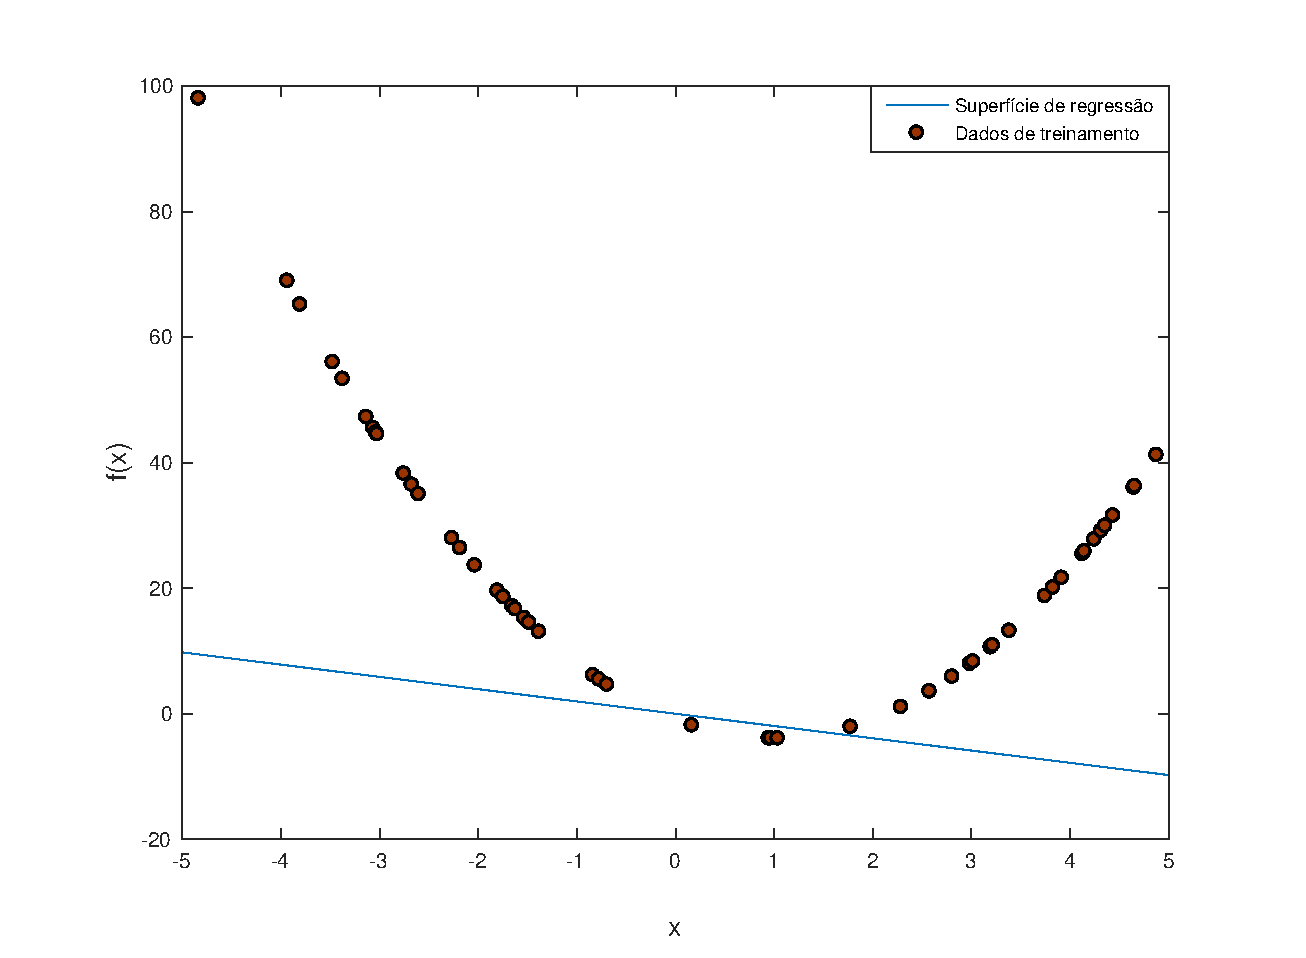
\includegraphics[width=.5\linewidth]{chapter1/linear.eps}
    \begin{center}
        \makebox[\width]{Fonte: Autor.}
    \end{center}
\end{figure}

O truque do \textit{kernel} pode ser visto como um atalho computacional que traz duas grandes vantagens: (\textit{i}) permite a criação de extensões (não-lineares) de métodos lineares; e (\textit{ii}) não exige demasiados recursos computacionais, pois não é necessário o cômputo do mapeamento de forma explícita. Não à toa, esses métodos tornaram-se tão populares em problemas de regressão \cite{shawe2004}. A Figura \ref{fig:ch1-poly} exemplifica bem o poder do truque do \textit{kernel}, onde predições mais precisas são realizadas ao utilizar uma mapeamento dos dados com uma função polinomial, e aplicando o método KRR. Mais informações sobre KRR e o truque do \textit{kernel} podem ser obtidas no Capítulo \ref{chapter:kernel-methods}.

\begin{figure}[H]
    \centering
    \caption{Resultado da predição obtida pelo modelo KRR com uma função de mapeamento polinomial.}
    \label{fig:ch1-poly}
    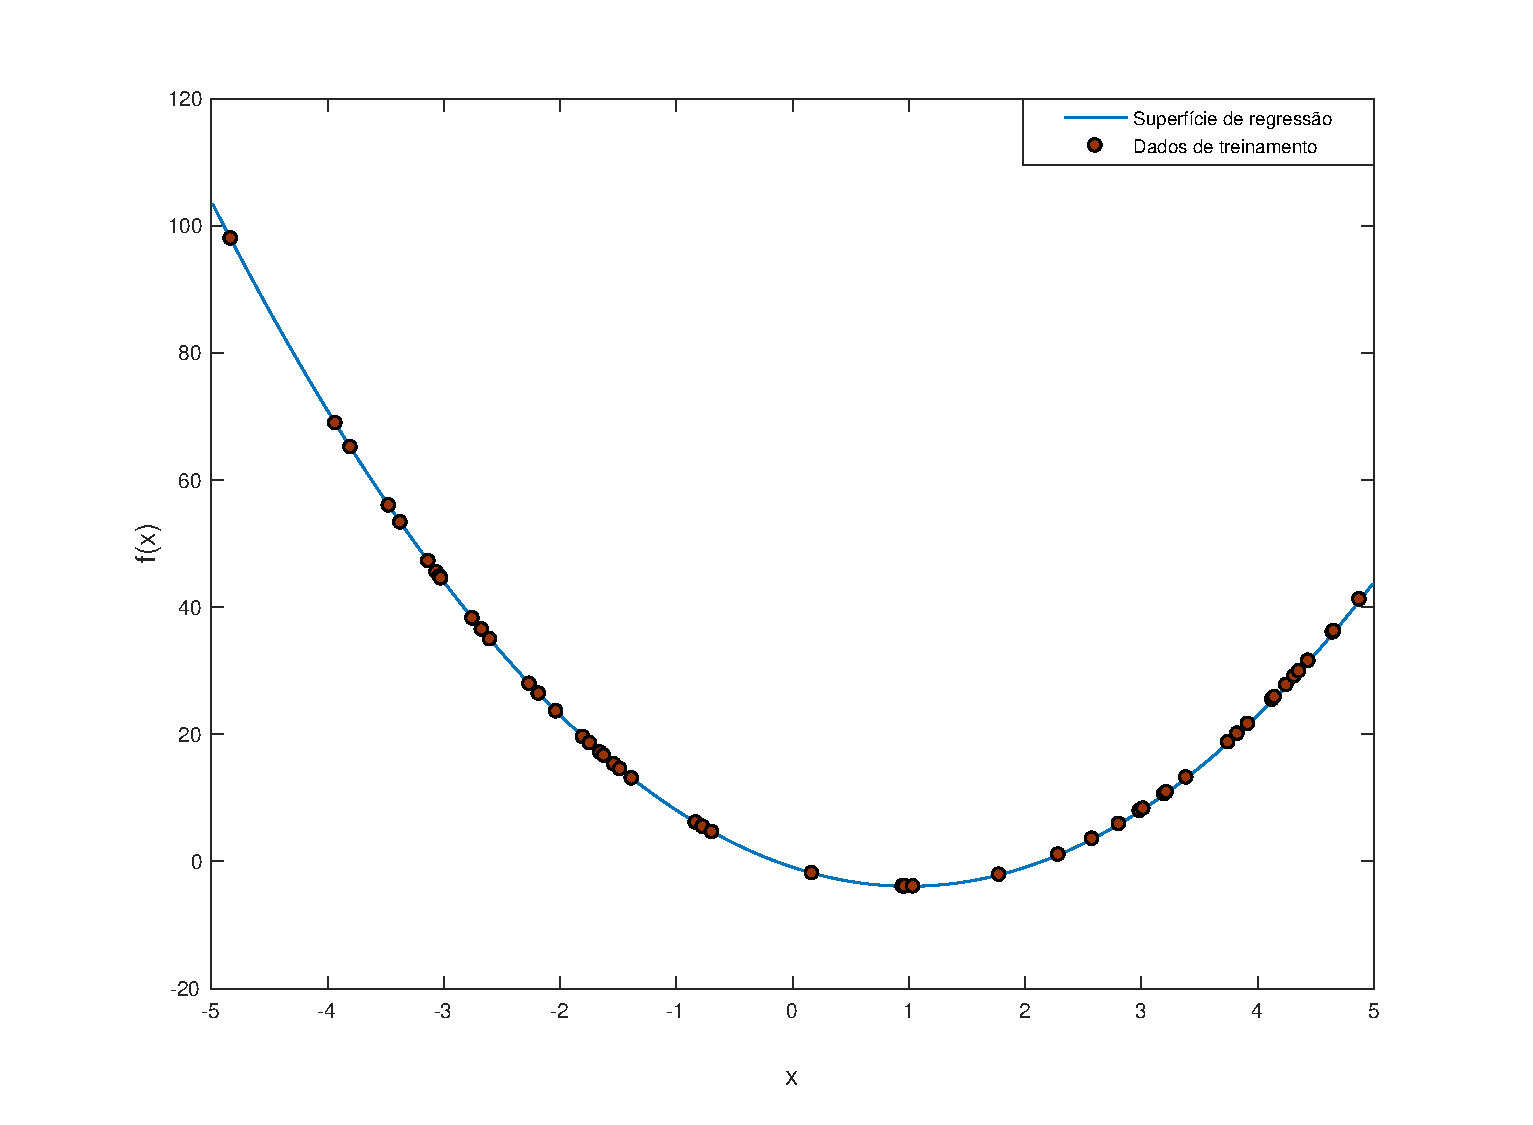
\includegraphics[width=.5\linewidth]{chapter1/poly.eps}
    \begin{center}
        \makebox[\width]{Fonte: Autor.}
    \end{center}
\end{figure}

\clearpage

Deste modo, em tarefas de regressão baseada em métodos de \textit{kernel}, o objetivo é encontrar uma função que mapeie os dados originalmente não-lineares, para um espaço onde estes apresentem-se linearmente \cite{smola1998}. Encontrar tal função é uma tarefa árdua, tanto que muitos pesquisadores optam por utilizar \textit{kernels} clássicos, tais como \textit{rbf} e polinomial, otimizando apenas seus parâmetros. Contudo, essa abordagem resulta em variações no desempenho para diferentes conjuntos de dados \cite{howley2005}. Criar funções de \textit{kernel} que se adaptem a um determinado conjunto de dados é uma solução mais conveniente e tornou-se um tópico de muito interesse da comunidade acadêmica, sendo chamado também de ``tópico quente'' (do inglês, \textit{hot topic}).

% \section{Trabalhos relacionados} \label{sec:related-work}
Técnicas de Computação Evolucionária (CE), como Programação Genética (PG), têm sido bastante utilizadas na criação automática de novas funções de \textit{kernel} em diferentes classes de problemas. Entretanto, na maioria destes estudos, técnicas de PG são aplicadas em tarefas de classificação utilizando Máquinas de Vetores Suporte (\textit{Support Vector Machines}, SVM). O primeiro trabalho que se tem registro da utilização de PG para criação de novos \textit{kernels} foi proposto por \citeonline{howley2005}. Neste, os autores utilizam a evolução em paralelo de cinco populações (de \textit{kernels}) com o objetivo de eliminar o teste de várias combinações de parâmetros. Ao fim do processo, o indivíduo mais apto de todas as populações é escolhido como o \textit{kernel} utilizado na criação do modelo final.

Em \cite{howley2006}, os autores reconhecem a capacidade de criação automática de novos \textit{kernels} e focam seu uso especificamente para classificadores SVM. As diferenças primordiais entre esta proposta e a anterior encontram-se numa representação mais sofisticada do \textit{kernel}, função de aptidão baseada em validação cruzada e um filtro de Mercer (se um \textit{kernel} não obedece ao teorema, recebe o valor mais baixo de aptidão).

\citeonline{diosan2007} utilizam um conjunto de operadores maior que \cite{howley2006}, incluindo operadores que transformam o espaço $\mathbb{R}^p$ no espaço $\mathbb{R}$. Entretanto, os autores não garantem que os \textit{kernels} criados obedeçam ao teorema de Mercer. Apesar disso, os resultados obtidos são bons e possuem um desempenho ligeiramente superior aos \textit{kernels} clássicos.

\citeonline{sullivan2007} utilizam uma técnica de PG conhecida como \textit{Strongly-Typed Genetic Programming} (STGP) para garantir que cada nó da árvore possa ter somente um determinado conjunto de operadores e/ou terminais como candidatos a nós-filho. Essa técnica permite que o \textit{kernel} gerado obedeça ao teorema de Mercer.

\citeonline{girdea2007} utilizam apenas combinações dos kernels linear, \textit{rbf} e polinomial na construção de novos \textit{kernels}. Além disso, o fator que o diferencia dos demais trabalhos é o uso de um meta-algoritmo conhecido como \textit{boosting}, que tem como objetivo combinar os resultados de classificadores mais ``fracos'' para formar um classificador mais preciso. Em particular, é utilizado o algoritmo InfoBoost \cite{aslam2000}.

\citeonline{alizadeh2011} apresentam uma abordagem diferente das anteriores. Os \textit{kernels} construídos durante o processo evolutivo são utilizados como entradas dos \textit{kernels} linear e \textit{rbf}. A partir destes, a classificação é efetuada. Os resultados confirmam uma superioridade de desempenho sobre os \textit{kernels} clássicos. Contudo, para conjuntos de dados de alta dimensão, o espaço de busca pelo \textit{kernel} ideal torna-se inviável. Os autores propõem mapear os dados de entrada para espaços de menor dimensão que o original, porém com mais de uma dimensão. Tal proposta não foi investigada e, assim, o trabalho dos autores não alcança o desempenho almejado (se comparado aos trabalhos anteriores).

Outro trabalho interessante que aplica PG para combinação de kernels foi proposto por \citeonline{schuh2012}, que utilizam Enxame de Partículas (\textit{Particle Swarm Optimization}, PSO) como fator adicional no processo de evolução. A combinação de \textit{kernels} é também aplicada em problemas específicos, como classificação de imagens \cite{ribeiro2015}, classificação de sequências de DNA hipersensíveis \cite{kamath2011} e classificação de padrões em expressão de genes \cite{cuong2006}.

Enquanto os trabalhos descritos nos parágrafos anteriores focam suas aplicações para tarefas de classificação (genéricas e específicas), não foram encontradas aplicações em problemas de regressão. Dessa forma, este trabalho propõe a criação de novas funções de \textit{kernel} a partir de outras preexistentes aplicadas em problemas de regressão, visto ser uma área pouco explorada. Para alcançar esse objetivo, é utilizado PG para combinação das funções de \textit{kernel} de base. Através do uso de propriedades de construção de novos \textit{kernels}, em conjunto com uma representação genética de STGP podemos garantir que as funções geradas obedecem ao teorema de Mercer. Para fins de avaliação, a proposta é comparada a métodos estado-da-arte, tais como Regressão de Vetores Suporte (\textit{Support Vector Regression}, SVR) e Redes Neurais Artificiais (RNA) do tipo MLP e RBF.

\section{Objetivos Geral e Específicos}
Este trabalho tem como objetivo geral propor uma técnica de criação automática de novas funções de \textit{kernel} adaptáveis para problemas de regressão. Para alcançar esse objetivo deve-se utilizar PG para criar combinações de funções já conhecidas. Através dessas combinações, o método garante adaptabilidade ao criar \textit{kernels} específicos para cada problema.

Mais particularmente, este trabalho possui os seguintes objetivos específicos:

\begin{itemize}
	\item Avaliar o desempenho do método proposto em realizar predições para problemas de regressão, assim como seu tempo médio de execução.
    \item Avaliar o uso de um determinado conjunto de funções de \textit{kernel} como base do processo de combinação e evolução, para criação de novos \textit{kernels}.
    \item Criar um mecanismo de geração automática de funções de \textit{kernel} que melhor se adaptem a um determinado problema.
    \item Comparar o desempenho do método proposto com o de métodos estado-da-arte, como SVR e Redes Neurais Artificiais.
    \item Verificar e validar a aplicação da \textit{ridge regression} no espaço de características gerado pelas funções de \textit{kernels} criadas.
\end{itemize}

\section{Estrutura da Monografia}
Esta monografia é composta de cinco capítulos -- além deste --, organizados da seguinte forma: fundamentos de programação genética; métodos de \textit{kernel} para regressão, incluindo o modelo proposto; simulações computacionais; conclusões e trabalhos futuros.

De modo geral, os Capítulos \ref{chapter:genetic-programming} e \ref{chapter:kernel-methods} apresentam os fundamentos teóricos necessários para o entendimento deste trabalho. No Capítulo \ref{chapter:genetic-programming} são descritos os principais conceitos sobre o arcabouço de PG. O nível de detalhes, uso de figuras para exemplificação ajudarão na definição do modelo GKR. O Capítulo \ref{chapter:kernel-methods} apresenta o conceito de regressão linear e o uso dos mínimos quadrados para estimação dos coeficientes de regressão. Apresenta ainda uma versão mais genérica da regressão linear, chamada de \textit{ridge regression}, que realiza um balanceamento entre a norma e o erro. A última seção de fundamentos teóricos deste capítulo apresenta a formulação dual e como a partir desta, surge naturalmente a ideia de funções de \textit{kernel}. Na última seção do Capítulo \ref{chapter:kernel-methods} é apresentada a proposta deste trabalho, denominada GKR.

No Capítulo \ref{chapter:simulations} são apresentadas a metodologia utilizada, as simulações computacionais e os resultados obtidos, além das respectivas discussões. São utilizados problemas de natureza artificial e real. Os problemas de natureza artificial auxiliam na prova de conceito acerca do funcionamento do modelo proposto, enquanto os problemas de natureza real auxiliam na análise de desempenho do modelo em solucionar problemas do mundo real. São apresentadas tabelas com o RMSE e tempo totais (treinamento e teste) médios, assim como gráficos dos valores de aptidão médios ao longo das gerações.

O Capítulo \ref{chapter:conclusions} são apresentadas as conclusões e considerações finais sobre este trabalho. Por fim, é apresentada uma proposta de trabalho futuro.